% !Mode\dots ``TeX:UTF-8''
% !TEX root = ../bare_jrnl.tex


\section{Introduction}
\label{sec:intro}


\IEEEPARstart{I}n 1960s, Nobel Prize laureates Jacob and Monod~\cite{Jacob1961Genetic} found that ``Any cell contains a number of regulatory genes that act as switches and can turn one another on and off. If genes can turn one another on and off, then you can have genetic circuits.'' Inspired by these Boolean-type actions in genetic circuits, Boolean networks (\BNs) were firstly proposed by Kauffman \cite{Kauffman1968Metabolic} for modeling nonlinear and complex biological systems. 

{\BNs} are a type of discrete-time dynamical systems which can be represented as directed graphs. In a BN, each node has only two values ``0" and ``1", and they can change in different time steps.  For a node $n_i$, we use $n_i(t)$ to denote the value of $n_i$ at the time step $t$.
In general, $n_i(t+1)$ is determined by a logical function of $n_j(t),\ldots,n_p(t)$ if  there are  edges from $n_j,\ldots,n_p$ to $n_i$.  
%The logical operators used in  the logical functions include AND, OR, NO, XOR.  
Some general descriptions of the \BNs\ and their applications to biological systems can be found in~\cite{Kauffman1968Metabolic}. There are many both natural and artificial systems works~\cite{Akutsu2000Inferring, Shmulevich2002From, Faur2006Dynamical,Green2007The,Lou2010Multi} related to \BNs.
 

\BNs\ can be naturally extended to Boolean control networks (\BCNs) when external regulations or perturbations are considered~\cite{Ideker2001A}. There are three kinds of nodes in \BCNs, including input-nodes ($\mathsf{i}$), state-nodes ($\mathsf{s}$) and output-nodes ($\mathsf{o}$). In \BCNs, we can only control input-nodes and observe output-nodes. 

For each state-node, $\mathsf{s}_i(t+1)$ is decided by a logical function of  $\{\mathsf{s}_j(t),\ldots,\mathsf{s}_p(t),\mathsf{i}_x(t),\ldots,\mathsf{i}_y(t)\}$  %if there are directed edges from $
while each $\mathsf{o}_i(t)$ is decided by a logical function of   $\{\mathsf{s}_j(t),\ldots,\mathsf{s}_p(t)\}$. 

\BCNs\ can be used to solve various real-life problems, for instance, 
structural and functional analysis of signalling and regulatory networks~\cite{Kaufman1999A, Klamt2006A}, 
abduction based drug target discovery~\cite{Biane2017Abduction}, 
and pursuing evasion problems in polygonal environments~\cite{Thunberg2011A}. 

We are mainly interested in the control-theoretic problems of \BCNs. The work~\cite{Akutsu2007Control} proves that the problem of determining the controllability of \BCNs\ is {\bf NP}-hard in the number of nodes. In addition, it points out that ``One of the major goals of systems biology is to develop a control theory for complex biological systems.'' Since then, the study on control-theoretic problems in the areas of \BNs\ and \BCNs\ has drawn great attention \cite{cheng2009controllability, Zhao2010Input, Cheng2011Identification, Cheng2011Analysis,Fornasini2013Observability}. What is more, the controllability and observability are the basic control-theoretic problems of \BCNs. % Among these studies, \emph{semi-tensor product} (\STP) is one of useful tools to deal with  

In this paper, we investigate the observability of \BCNs. The concept of observability was proposed firstly in~\cite{cheng2009controllability}. To date, there are four types of observability proposed in the literature. And they are mainly about determine the initial value of the state-nodes of the \BCNs\ by the value of their input-nodes and output-nodes. 

The vectors input $\mathsf{i}(t)=[\mathsf{i}_1(t)\ldots\mathsf{i}_m(t)]^T$, state $\mathsf{s}(t)=[\mathsf{s}_1(t) \ldots \mathsf{s}_n(t)]^T$ and output $\mathsf{o}(t)=[\mathsf{o}_1(t) \ldots \mathsf{o}_q(t)]^T$ represent the value of all input-nodes, all state-nodes and all output-nodes, respectively, where $m$, $n$ and $q$ represent the number of input-nodes, state-nodes and output-nodes, respectively. 
 Then $\mathsf{s}(t+1)$ is decided by $\mathsf{i}(t)$ and $\mathsf{s}(t)$, and $\mathsf{o}(t)$ is decided by $\mathsf{s}(t)$ as shown in Fig.~\ref{fig:10}.


 \begin{figure}[!t]
      \centering
      \framebox{\parbox{3in}{
		\centerline{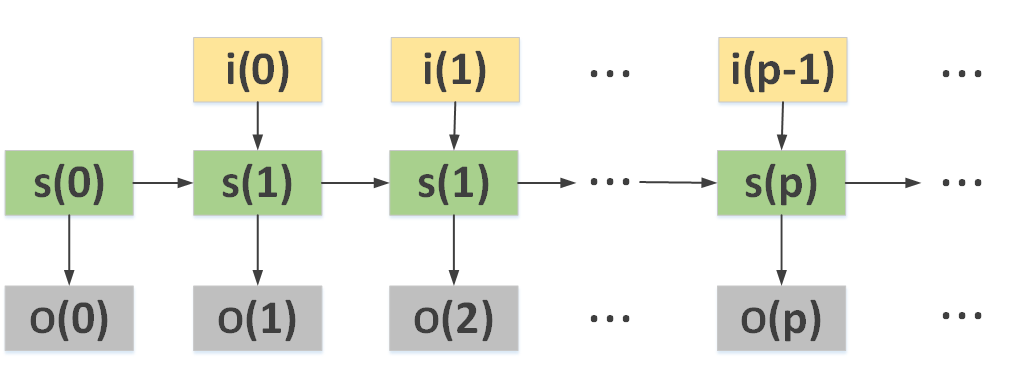
\includegraphics[scale=0.17]{figures/Fig10.png}}
	}}
      
      \caption{The relationship of inputs, states and outputs.}
      \label{fig:10}
  \end{figure}
   The sequences $\mathsf{i}(0)\mathsf{i}(1)\ldots\mathsf{i}(k-1)$,  $\mathsf{s}(0)\mathsf{s}(1)\ldots\mathsf{s}(k)$, and $\mathsf{o}(0)\mathsf{o}(1)\ldots\mathsf{o}(k)$ 
 consists of several inputs, states and outputs in sequential time steps,  respectively, where $k>0$. 
 Such that, for an initial state $\mathsf{s}(0)$ and a  sequence of inputs $\mathsf{i}(0)\mathsf{i}(1)\ldots\mathsf{i}(k-1)$ of a \BCN, we have its corresponding 
$\mathsf{s}(0)\mathsf{s}(1)\ldots\mathsf{s}(k)$ and $\mathsf{o}(0)\mathsf{o}(1)\ldots\mathsf{o}(k)$.  
%That is for a given  \BCN\  $\BB$,  $\mathsf{o}(0)\mathsf{o}(1)\ldots\mathsf{o}(k)$ is decide by $\mathsf{s}(0)$ and the sequence $\mathsf{i}(0)\mathsf{i}(1)\ldots\mathsf{i}(k-1)$. 
And we use $\mathsf{s}^{x}(t)$ and $\mathsf{s}^{y}(t)$ to represent different valuations of $\mathsf{s}(t)$, and similarly for input-nodes and output-nodes. Then the four existing observability of \BCNs\ can be described as follows. 

\begin{enumerate}
	\item The first type of observability was proposed in 2009 \cite{cheng2009controllability}, and it states that a \BCN\ $\BB$ is observable if for every $\mathsf{s}^{x}(0)$ there is an $\mathsf{i}(0)\mathsf{i}(1)\ldots\mathsf{i}(k-1)$ that can be used to distinguish $\mathsf{s}^{x}(0)$ from other types of initial states. That is in the $\BB$, for the $\mathsf{s}^{x}(0)$ and $\mathsf{i}(0)$$\mathsf{i}(1)\ldots$$\mathsf{i}(k-1)$, we have for every $\mathsf{s}^{y}(0)\ne\mathsf{s}^{x}(0)$, the corresponding $\mathsf{o}^{y}(0)$$\mathsf{o}^{y}(1)\ldots$$\mathsf{o}^{y}(k)$ of $\mathsf{s}^{y}(0)$ is different from the corresponding $\mathsf{o}^{x}(0)$$\mathsf{o}^{x}(1)\ldots$$\mathsf{o}^{x}(k)$ of $\mathsf{s}^{x}(0)$. 
	%------------------------------
	\item 
	The second observability was proposed in 2010 \cite{Zhao2010Input}, and it is determined in \cite{Li2015Controllability}. It states that a \BCN\ $\BB$ is observable if for every two distinct $\mathsf{s}^{x}(0)$ and $\mathsf{s}^{y}(0)$, there exists an $\mathsf{i}(0)$$\mathsf{i}(1)\ldots$$\mathsf{i}(k-1)$ that can be used to distinguish them. That is in the $\BB$, for the $\mathsf{s}^{x}(0)$, $\mathsf{s}^{y}(0)$ and $\mathsf{i}(0)\mathsf{i}(1)\ldots\mathsf{i}(k-1)$, we have the corresponding $\mathsf{o}^{x}(0)\mathsf{o}^{x}(1)\ldots\mathsf{o}^{x}(k)$ of $\mathsf{s}^{x}(0)$ and the corresponding $\mathsf{o}^{y}(0)\mathsf{o}^{y}(1)\ldots\mathsf{o}^{y}(k)$ of $\mathsf{s}^{y}(0)$ are different.
	\item The third observability proposed in 2011 \cite{Cheng2011Identification}, and it states that a \BCN\ $\BB$ is observable if there is an $\mathsf{i}(0)$$\mathsf{i}(1)\ldots$$\mathsf{i}(k-1)$ that determines $\mathsf{s}(0)$. That is in the $\BB$, for the $\mathsf{i}(0)$$\mathsf{i}(1)\ldots$$\mathsf{i}(k-1)$, we have for every two distinct $\mathsf{s}^{x}(0)$ and $\mathsf{s}^{x}(0)$, the corresponding $\mathsf{o}^{x}(0)$$\mathsf{o}^{x}(1)\ldots$$\mathsf{o}^{x}(k)$ of $\mathsf{s}^{x}(0)$ is different from the corresponding $\mathsf{o}^{y}(0)$$\mathsf{o}^{y}(1)\ldots$$\mathsf{o}^{y}(k)$ of $\mathsf{s}^{y}(0)$.
	
	\item  The fourth observability proposed in 2013 \cite{Fornasini2013Observability} is essentially the observability of linear control systems, i.e., that a \BCN\ $\BB$ is observable if every sufficient long $\mathsf{i}(0)$$\mathsf{i}(1)\ldots$$\mathsf{i}(k-1)$ can determine $\mathsf{s}(0)$. That is in the $\BB$, we have for every sufficient long $\mathsf{i}(0)$$\mathsf{i}(1)\ldots$ $\mathsf{i}(k-1)$, for every two distinct $\mathsf{s}^{x}(0)$ and $\mathsf{s}^{y}(0)$, the corresponding $\mathsf{o}^{x}(0)$$\mathsf{o}^{x}(1)\ldots$$\mathsf{o}^{x}(k)$ of $\mathsf{s}^{x}(0)$ is different from the corresponding $\mathsf{o}^{y}(0)$$\mathsf{o}^{y}(1)\ldots$$\mathsf{o}^{y}(k)$ of $\mathsf{s}^{y}(0)$.
\end{enumerate}
 Their formal definitions will be presented in Section~\ref{sec:pre}.

 In the four notions of observability, the first and second one determine $\mathsf{s}(0)$ by taking the determining procedure multiple times, and the third and fourth one determine $\mathsf{s}(0)$ by taking the determining procedure once. %And the second observability is the necessary and sufficient condition of determining $\mathsf{s}(0)$ by taking the determining procedure once. 
 In this paper, we address the necessary and sufficient condition of determining $\mathsf{s}(0)$ by taking the determining procedure once.
\begin{itemize}
	\item It enriches the control-theory of \BCNs, it may help us further researching the identification of \BCNs. 
	\item And it can help us determine the $\mathsf{s}(0)$ of some \BCNs\ which can not be determined before.
\end{itemize}
%\begin{problem}
%\label{pro:1}
%For a given \BCN\ $\BB$, whether its initial state $\mathsf{s}(0)$ can be determined by carrying on determining procedure once?
%\end{problem}

%Although, these four existing notions of observability can help us study some information about $\mathsf{s}(0)$ we need. 
%The problem means that whether the $\mathsf{s}(0)$ can be determined if the determining procedure can do at most once. %only third and fourth ones  can  determine the $\mathsf{s}(0)$ of \BCNs.
%Only third and fourth notions of observability can help us solve the {\em Problem~\ref{pro:1}}.
% What is more, in the third observability, a \BCN\ is observable iff there is an input sequence that determines its initial state $\mathsf{s}(0)$. Thus its condition is very strong, and the condition of fourth observability is even stronger.
%However, 
We find that to determine $\mathsf{s}(0)$ by taking the determining procedure once we only need to complete the following procedure.

%Informly, the procedure of our  online observability as follows. 
For a given \BCN\  $\BB$, we use $\mathsf{S}(t)$ to denote the set of possible valuations of $\mathsf{s}(t)$. Then $\mathsf{S}(t)$ can be derived by the output sequence $\mathsf{o}(0)\mathsf{o}(1)\ldots\mathsf{o}(t)$, input sequence $\mathsf{i}(0)\mathsf{i}(1)\ldots\mathsf{i}(t-1)$ and updating rules of $\BB$.
\begin{itemize}
	\item  Firstly, at every time step we infer $\mathsf{S}(t)$ by the $\mathsf{o}(t)$ and the relation $\mathsf{o}(t)$ between $\mathsf{s}(t)$.
	\item Secondly, according to the relation of $\mathsf{i}(t)$, $\mathsf{s}(t)$ and $\mathsf{s}(t+1)$ we chose a $\mathsf{i}(t)$ which would not make every two distinct $\mathsf{s}^{x}(t)$ , $\mathsf{s}^{y}(t)$$\in$ $\mathsf{S}(t)$ become the same state after affected by $\mathsf{i}(t)$ i.e. $\mathsf{s}^{x}(t+1)\ne\mathsf{s}^{y}(t+1)$. Therefore, for every $\mathsf{s}^{x}(t+1)\in $ $\mathsf{S}(t+1)$ there is exact one corresponding $\mathsf{s}^{x}(t)\in $ $\mathsf{S}(t)$.
	\item Thirdly, we have $|$$\mathsf{S}(t)$$|\le|$$\mathsf{S}(t-1)$$|$. When $|$$\mathsf{S}(t)$$|=1$, we can determine $\mathsf{s}(t)$. Because for every $\mathsf{s}^{x}(t)\in $ $\mathsf{S}(t)$ there is exact one corresponding $\mathsf{s}^{x}(t-1)\in $ $\mathsf{S}(t-1)$ we can determine $\mathsf{s}(t-1)$, $\mathsf{s}(t-2)$,\ldots, and $\mathsf{s}(0)$.
\end{itemize}

%In the third observability, we can finish this procedure, thus we can determine the initial state \State$(0)$ for a \BCN. What is more, 
In this process, we do not have to get $\mathsf{i}(0)\mathsf{i}(1)\ldots\mathsf{i}(k-1)$ before taking the procedure of determining \State$(0)$. In other words, we can adaptively construct $\mathsf{i}(0)\mathsf{i}(1)\ldots\mathsf{i}(k-1)$ by every $\mathsf{S}(t)$ we derived.  
%Such that, the requirement for a \BCN\ to determine \State$(0)$ would be easist to satisfy. 
Inspired by this, we propose the online observability which states that a \BCN\ $\BB$ is observable if the $\mathsf{i}(0)\mathsf{i}(1)\ldots\mathsf{i}(k-1)$ to determine $\mathsf{s}(0)$ can be adaptively constructed. 

Comparing with the third and fourth observability, the online observability provides a dynamic approach to determine the initial states of \BCNs, such that the requirements for \BCNs\ to determine the initial state is easiest to satisfy. Thus it address the necessary and sufficient condition of determining $\mathsf{s}(0)$ by taking the determining procedure once.
Then, in this paper we make the following contributions. 
\subsubsection*{Contributions}
Firstly, we propose and formally define the online observability to address the necessary and sufficient condition of determining $\mathsf{s}(0)$ by taking the determining procedure once. %It enriches the control-theory of \BCNs. 
Secondly, in addition to theoretical research, we also provide determination algorithm for the online observability. Finally, we present some optimization brought by the online observability. Including the means to find shortest path and the approach to avoid entering critical states in the process of determining the initial states of \BCNs.  These optimization further explain the advantages of online observability of \BCNs. 

The remainder of this paper is organized as follows.

 {\em Section \ref{sec:pre}} introduces necessary preliminaries about \BCNs, including the definition of \BCNs\ and four existing observability. {\em Section \ref{sec:online}} presents the definition of online observability of \BCNs. {\em Section \ref{sec:deter}} presents determination algorithm for the online observability. 
% {\em Section \ref{sec:app}} talks about some optimization brought by the online observability of \BCNs. 
 {\em Section \ref{sec:con}} ends up with the introduction of our future work.

%==============================================================================================================